\chapter{Introduktion}
Vi vil indledningsvis præsentere konteksten for dette speciale. Herefter klarlægger vi, hvilke problemer vi ønsker at berøre samt hvad vores tilgangsvinkel er. Afslutningsvis giver vi et overblik over specialets struktur. 

\subsubsection{Kontekst}
Over de sidste par år er multi-kerne cpu'er blevet hyldevarer, hvilket har afledt et stigende behov for at udvikle programmer, der kan udnytte flere kerner samtidigt. Dette behov har gjort CSP til et populært sprog, da det gør det let at repræsentere samtidighed og desuden kræver eksplicit udveksling af data frem for at benytte delte datastrukturer, som kræver låsemekanismer eller anden form for kontrol over hvem der tilgår og hvordan det delte data tilgås. CSP's stigende popularitet har affødt at det er blevet blevet implementeret i flere andre programmeringssprog, og senest har Google lavet sproget Go, der er baseret på CSP. Med den stigende popularitet stiger behovet også for udviddet funktionalitet inden for niche-områder, heriblandt håndtering af tidsspecifikke problemer. Der er tidligere blevet arbejdet meget med at introducere tid i CSP, men det er primært på det teoretiske plan og har aldrig vundet indpas i de gængse implementationer. 

\subsubsection{Specialets problemformulering og struktur}
Set i lyset af den nuværende mangel på en praktisk anvendelig implementering af tid i CSP, vil vi undersøge om det er muligt at lave en sådan - dvs. en implementering, som kan bruges af udviklere til at løse problemer, hvori tid indgår.

For at opnå dette vil vi undersøge, hvad der skal til for at introducere følgende tre anvendelsesområder i \pycsp: Diskret simulering, realtids planlægning og interaktiv planlægning. Disse anvendelsesområder repræsenterer områder hvor tid indgår  og dækker tilsammen bredt over tid som helhed. Diskret simulering anvendes i stor udstrækning i discrete event simulation. Realtids planlægning benyttes i tidskritiske systemer hvor der er stringente krav om at en given begivenhed er blevet udført inden for en tidsramme. Endeligt bruges interaktiv planlægning i spilindustrien til at udregne scenen i et computerspil. På \cref{fig:intro} viser vi hvordan vi forventer at kombinere anvendelsområderne med \pycsp for derved at komme frem til vores Timed \pycsp. 

For hver model vil vi definere en række eksempler, der illustrerer disse anvendelsesområderne. Eksemplerne skal sikre den praktiske anvendelighed og senere bruges til at vise, hvordan et tidsspecifikt problem kan løses henholdsvis med og uden vores udvidelse. Eksemplernes formål er altså, at give et klart indblik i de krav, der stilles til en udvidelse af \pycsp, og hvilke fordele en introduktion af de givne anvendelsesområderne i \pycsp vil give. På denne baggrund vil vi komme med løsningsforslag som tager udgangspunkt i den praktiske anvendelighed. Disse løsningsforslag vil såfremt det er muligt, blive implementeret som en udvidelse af \pycsp.

Specialet vil derfor være struktureret som følger. I \autoref{chap:csp} vil vi gennemgå CSP og \pycsp med fokus på de dele der er relevante i forhold til at introducere tid. I \autorefs{chap:des}, \ref{chap:rtp} og \ref{chap:is} vil vi gennemgå de tre anvendelsesområder som beskrevet ovenfor. Afslutningsvis vil vi foretage en samlet i evaluering og konklusion i \autoref{chap:konklusion} på baggrund af delkonklusionerne i \autorefs{chap:des}, \ref{chap:rtp} og \ref{chap:is}.

\begin{figure}[htp]
 \begin{center}
  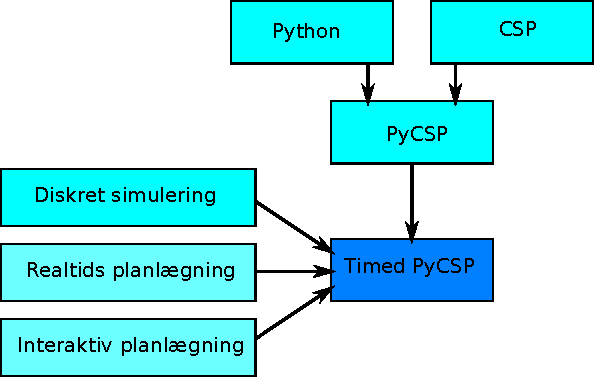
\includegraphics[scale=0.8]{images/intro}
	\caption{Samspil mellem CSP, Python og de tre tidsmodeller samlet i Timed \pycsp .}
	\label{fig:intro}
\end{center}
\end{figure}

%Mål: At lave en praktisk anvendelig udviddelse af pycsp, som kan bruges af udviklere til at løse problemer, der har en naturlig dimension af tid.

%Mål: At undersøge om det er muligt at lave en praktisk anvendelig udviddelse af pycsp, som kan bruges af udviklere til at løse problemer, der har en naturlig dimension af tid.

%\section{Vores bidrag}
%\section{Termer}

%\begin{list}{}{}
%\tightlist
%\item Scheduler findes ikke som et dansk ord, som kan  dække helt det samme. Vi har valgt at bruge ordet skemaplanlægger.
%\item I \des beskriver det enkelte \code{event} en begivenhed, og vi vil i dette speciale bruge ordet begivenhed for en event i \des. 
%\item realtid: tid mål i sekunder, minutter osv. TODO: TJEK FOR reel tid.
%\item simulering ikke simulation
%\item implementering ikke implementation.
%\item event: begivenhed
%\item Vi har fra koden der vises fjernet kode der ikke er relevant for sammenhængen, som f.eks kald til logging. Linje nr. vil derfor ikke altid passe, men det første linje nr i kodestumpen vil svare til linjenr i source koden.
%\item hvad skal emphs og hvad skal med stå med code osv.
%\item TODO: vi skal søge og styr på  greenlet vs. greenlets
%\item søg igennem grenelts og varianter
%\item SKIP-guard, skip-guard \code{skip-guard}? træf et valg mht. både skip og timeout. 
%\end{list}


%Vi vil bruge tekst markeret med \code{skrivemaskine-font} til at markere variabelnavne, funktioner,  klasser og moduler  der er  der er specifikt for Python.

